\documentclass[11pt]{article}
\usepackage[margin=1.5in]{geometry}
\usepackage{graphicx}
\usepackage{float}
\usepackage{parskip}
\usepackage{amsmath}
\usepackage{subfigure}
\usepackage{ulem}
\usepackage{pgfplots}
\usepgfplotslibrary{polar}
\pgfplotsset{width=10cm, compat=1.9}

\begin{document}

\textbf{\Huge Polar Coordinates and Complex Numbers}

Athan Zhang \& Jeffrey Chen

\section{Polar Coordinates}

Previously, we only dealt with Cartesian coordinates; you're typical $(x, y)$ points. This rectangular system is easy to understand and visualize. However, there are many applications where this rectangular system can be more cumbersome than need me. For example, in higher-level mathematics and physics, we often have to model systems that may be cylindrical, such as the volume of a can-shaped object or the trajectory of planets in orbit. In these examples, it is much easier to establish a new coordinate system to understand the relationship of position better.

In the rectangular coordinate system, the $x$ and $y$ axis are horizontal and vertical lines, respectively. Their intersection is called the origin, and the location of a point is given by its distance from the two axes.

In a polar coordinate system, there is a fixed origin called the \textbf{pole}. The \textbf{polar axis} is an initial ray that stems from the pole and it can be analogous to the positive x-axis. The location of the point is given by the \textbf{polar coordinates} of the point, which is composed of $r$, the directed distance from the origin to the point, and $\theta$, which is the angle made from $\overrightarrow{OP}$ and the polar axis.

\begin{figure}[H]
    \centering
    \includegraphics[width=0.6\textwidth]{Precalc/images/polar_coord.png}
\end{figure}

Remember that a positive $\theta$ denotes a counter-clockwise rotation while a negative $\theta$ denotes a clockwise rotation.

\subsection{Non-Unique}

In Cartesian coordinates, each point in space has exactly one unique Cartesian coordinate. However, this is not true in Polar coordinates. For example, we previously learned that an angle has infinitely many coterminal angles by simply adding some multiple of the periodicity of the angle. Additionally, we know that each angle has a corresponding negative angle that gives the same angular displacement on a circular coordinate system. Furthermore, the value of $r$ can be negative. Without considering coterminal angles, there are \textbf{four} ways to represent a single point with Polar coordinates.

\subsection{Conversion to Rectangular}

Unsurprisingly, we can use basic trigonometry to convert between Rectangular and Polar coordinates.

\textbf{Polar to Rectangular}
\begin{align*}
    x &= r\cos\theta \\
    y &= r\sin\theta \\
\end{align*}

\textbf{Rectangular to Polar}
\begin{align*}
    r &= \sqrt{x^2 + y^2} \\
    \theta &= \tan^{-1}\frac{y}{x} \\
\end{align*}
Recall that the domain of the arctan function is only from $[-90, 90]$ degrees, which corresponds to Quadrant I and Quadrant IV. If our point is in Quadrant II or Quadrant III, we must add 180 degrees or $\pi$ radians to our value for $\theta$.

\section{Graphing Polar Equations}

An equation expressed in terms of polar coordinates is called a polar equation. For example, $r = 2\sin\theta$ is a polar equation. A polar graph is the graphical representation of the set of all points with polar coordinates that satisfy the polar equation.

To graph polar equations, plug-in points for $\theta$. Make sure to extend your range as necessary.

\subsection*{Symmetry}

Polar graphs can be symmetric with respect to the polar axis (x-axis), $\theta = \pi/2$ (y-axis), and origin. Some quick tests for symmetry:
\begin{itemize}
    \item \textbf{Polar Axis:} It is a function of $\cos\theta$
    \item $\mathbf{\theta = \pi/2:}$ It is a function of $\sin\theta$
\end{itemize}

\subsection{Circles}

There are multiple ways to represent circles with polar coordinates. The easiest is to simply set $r$ to be some constant. This will produce a circle centered at the polar pole. The other two methods involve the $\cos$ and $\sin$ trigonometric functions.

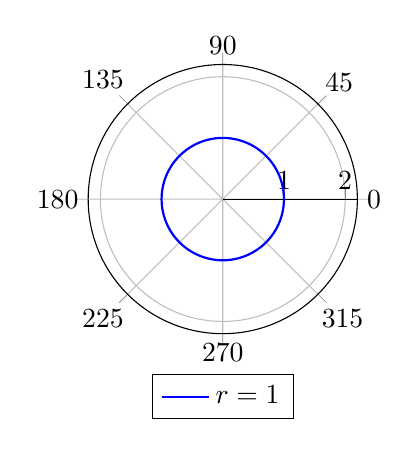
\begin{tikzpicture}

    % Fig 1
    \begin{polaraxis}[
        width=5cm, 
        height=5cm,
        domain=0:360, 
        range=0:2,
        ymax=2.2,
        samples=200,
        legend style={at={(0.5,-0.15)}, anchor=north},
        ytick={1,2}
    ]
    \addplot[blue, thick] {1}; 
    \addlegendentry{$r = 1$}
    \end{polaraxis}
    \hspace{5cm}
    
    % Fig 2
    \begin{polaraxis}[
        width=5cm, 
        height=5cm,
        domain=0:360, 
        samples=200,
        legend style={at={(0.5,-0.15)}, anchor=north},
        ytick={1,2}
    ]
    \addplot[blue, thick] {2*sin(x)}; 
    \addlegendentry{$r = 2\sin\theta$}
    \end{polaraxis}
    \hspace{5cm}
    
    % Fig 3
    \begin{polaraxis}[
        width=5cm, 
        height=5cm,
        domain=0:360, 
        samples=200,
        legend style={at={(0.5,-0.15)}, anchor=north},
        ytick={1,2}
    ]
    \addplot[blue, thick] {2*cos(x)}; 
    \addlegendentry{$r = 2\cos\theta$}
    \end{polaraxis}
\end{tikzpicture}

The last two equations can be generalized to the form 
\begin{align*}
    r &= a\cos \theta \\
    r &= a\sin \theta \\
\end{align*}
If $a > 0$, then the circles are oriented toward the corresponding positive $x$ and $y$ axis. If $a < 0$, then it is in the negative direction.

\subsection{Lines}

We can derive the polar equation of a line by using the conversion of polar and rectangular coordinates.

\begin{align*}
    y &= mx + b \\
    r\sin\theta &= mr\cos\theta + b \\
    r(\sin\theta - m\cos\theta) &= b \\
    r &= \frac{b}{(\sin\theta - m\cos\theta)}
\end{align*}

However, we notice that when $b = 0$, which means the line passes through the origin, there is no plausible equation. In this case, it is much easier to set $\theta$ equal to some constant angle.

\begin{tikzpicture}

    % Fig 1
    \begin{polaraxis}[
        width=5cm, 
        height=5cm,
        domain=0:1000, 
        samples=1000,
        ymax=2.2,
        legend style={at={(0.5,-0.15)}, anchor=north},
        ytick={1,2}
    ]
    \addplot[blue, thick] {0.1 / (sin(x) + cos(x))}; 
    \addlegendentry{$\theta = -\pi/4$}
    \end{polaraxis}
    \hspace{5cm}
    
    % Fig 2
    \begin{polaraxis}[
        width=5cm, 
        height=5cm,
        domain=-1000:1000, 
        ymax=2.2,
        samples=1000,
        legend style={at={(0.5,-0.15)}, anchor=north},
        ytick={1,2}
    ]
    \addplot[blue, thick] {3/(sin(x)-3*cos(x))}; 
    \addlegendentry{$r = \frac{3}{\sin\theta - 3\cos\theta}$}
    \end{polaraxis}
    \hspace{5cm}

    % Fig 3
    \begin{polaraxis}[
        width=5cm, 
        height=5cm,
        domain=-1000:1000, 
        ymax=2.2,
        samples=1000,
        legend style={at={(0.5,-0.15)}, anchor=north},
        ytick={1,2}
    ]
    \addplot[blue, thick] {-1/(sin(x)+0.2*cos(x))}; 
    \addlegendentry{$r = \frac{-1}{\sin\theta + 0.2\cos\theta}$}
    \end{polaraxis}
\end{tikzpicture}

\subsection{Limaçons}

Limaçons are of the form
\begin{align*}
    r &= a \pm b\cos\theta \\
    r &= a \pm b\sin\theta \\
\end{align*}
where both $a$ and $b$ are positive. There are four types of Limaçons. The types of Limaçons are determined by the relationship between $a$ and $b$. 

An interesting property of a Limaçon is that we can calculate its width/height (the distance from the origin to the furthest point on the Limaçon) as $a+b$. We can also calculate the width/height of its inner-loop (if there is one) as $b - a$.

Notice in the display of the four types, we also explore the combinations in Limaçons with $\pm$ and $\cos$ or $\sin$.

\subsubsection*{Inner-Loop Limaçon}

An Inner-Loop Limaçon is found when $a < b$.

\begin{center}
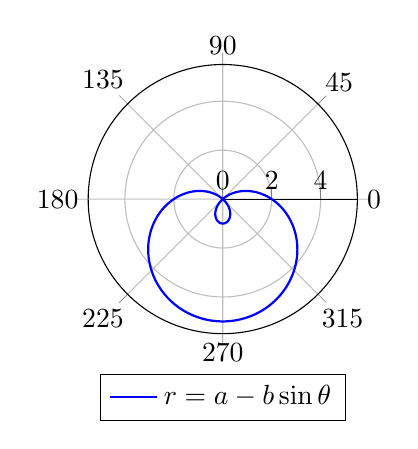
\begin{tikzpicture}
    \begin{polaraxis}[
        width=5cm, 
        height=5cm,
        domain=0:360, 
        samples=200,
        legend style={at={(0.5,-0.15)}, anchor=north},
    ]
    \addplot[blue, thick] {2 - 3*sin(x)}; 
    \addlegendentry{$r = a - b\sin\theta$}
    \end{polaraxis}
\end{tikzpicture}
\end{center}

\subsubsection*{Cardioid}

A Cardioid (heart-shaped) is found when $a = b$.

\begin{center}
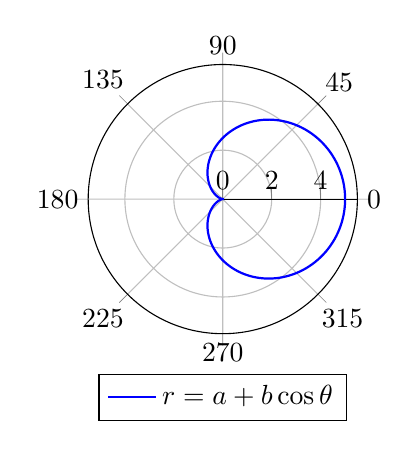
\begin{tikzpicture}
    \begin{polaraxis}[
        width=5cm, 
        height=5cm,
        domain=0:360, 
        samples=200,
        legend style={at={(0.5,-0.15)}, anchor=north},
    ]
    \addplot[blue, thick] {2.5 + 2.5*cos(x)}; 
    \addlegendentry{$r = a + b\cos\theta$}
    \end{polaraxis}
\end{tikzpicture}
\end{center}

\subsubsection*{Dimpled Limaçon}

A Dimpled Limaçon is found when $b < a < 2b$.

\begin{center}
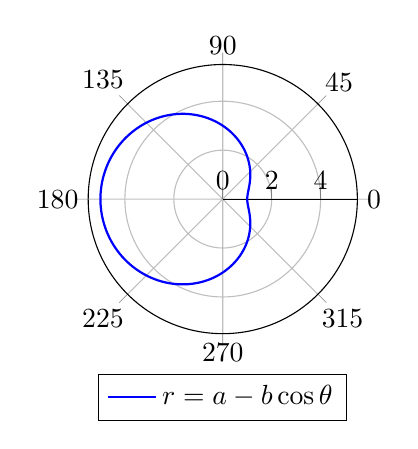
\begin{tikzpicture}
    \begin{polaraxis}[
        width=5cm, 
        height=5cm,
        domain=0:360, 
        samples=200,
        legend style={at={(0.5,-0.15)}, anchor=north},
    ]
    \addplot[blue, thick] {3 - 2*cos(x)}; 
    \addlegendentry{$r = a - b\cos\theta$}
    \end{polaraxis}
\end{tikzpicture}
\end{center}

\subsubsection*{Convex Limaçon}

An Convex Limaçon is found when $a \geq 2b$.

\begin{center}
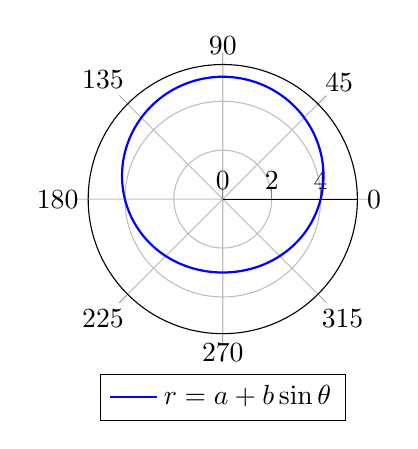
\begin{tikzpicture}
    \begin{polaraxis}[
        width=5cm, 
        height=5cm,
        domain=0:360, 
        samples=200,
        legend style={at={(0.5,-0.15)}, anchor=north},
    ]
    \addplot[blue, thick] {4 + 1*sin(x)}; 
    \addlegendentry{$r = a + b\sin\theta$}
    \end{polaraxis}
\end{tikzpicture}
\end{center}

\subsection{Roses}

Roses are of the form
\begin{align*}
    r &= a\cos n\theta \\
    r &= a\sin n\theta \\
\end{align*}
where $n \geq 2$ and is an integer. The value of $a$ gives the length of one petal, which is the distance from the polar pole to the tip of a single petal.

\subsection*{Odd-n Roses}

Roses with an odd-numbered $n$ have $n$ petals.

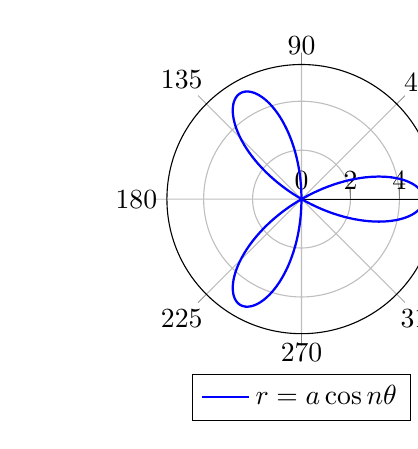
\begin{tikzpicture}
    \hspace{1cm}
    \begin{polaraxis}[
        width=5cm, 
        height=5cm,
        domain=0:360, 
        samples=200,
        legend style={at={(0.5,-0.15)}, anchor=north},
    ]
    \addplot[blue, thick] {5*cos(3*x)}; 
    \addlegendentry{$r = a\cos n\theta$}
    \end{polaraxis}
    \hspace{7cm}
    \begin{polaraxis}[
        width=5cm, 
        height=5cm,
        domain=0:360, 
        samples=200,
        legend style={at={(0.5,-0.15)}, anchor=north},
    ]
    \addplot[blue, thick] {5*sin(5*x)}; 
    \addlegendentry{$r = a\sin n\theta$}
    \end{polaraxis}
\end{tikzpicture}

\subsection*{Even-n Roses}

Roses with an even-numbered $n$ have $2n$ petals.

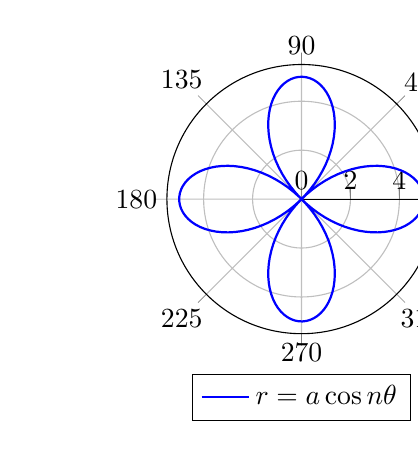
\begin{tikzpicture}
    \hspace{1cm}
    \begin{polaraxis}[
        width=5cm, 
        height=5cm,
        domain=0:360, 
        samples=200,
        legend style={at={(0.5,-0.15)}, anchor=north},
    ]
    \addplot[blue, thick] {5*cos(2*x)}; 
    \addlegendentry{$r = a\cos n\theta$}
    \end{polaraxis}
    \hspace{7cm}
    \begin{polaraxis}[
        width=5cm, 
        height=5cm,
        domain=0:360, 
        samples=200,
        legend style={at={(0.5,-0.15)}, anchor=north},
    ]
    \addplot[blue, thick] {5*sin(4*x)}; 
    \addlegendentry{$r = a\sin n\theta$}
    \end{polaraxis}
\end{tikzpicture}

\subsection{Lemniscates}

Lemniscates are of the form
\begin{align*}
    r^2 &= a^2 \cos 2\theta \\
    r^2 &= a^2 \sin 2\theta \\
\end{align*}

Where $a$ is the length of a petal.

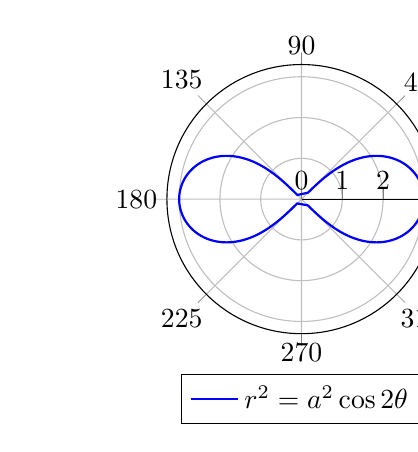
\begin{tikzpicture}
    \hspace{1cm}
    \begin{polaraxis}[
        width=5cm, 
        height=5cm,
        domain=0:360, 
        samples=2000,
        legend style={at={(0.5,-0.15)}, anchor=north},
    ]
    \addplot[blue, thick] {(9*cos(2*x))^0.5}; 
    \addlegendentry{$r^2 = a^2\cos 2\theta$}
    \end{polaraxis}
    \hspace{7cm}
    \begin{polaraxis}[
        width=5cm, 
        height=5cm,
        domain=0:360, 
        samples=2000,
        legend style={at={(0.5,-0.15)}, anchor=north},
    ]
    \addplot[blue, thick] {(9*sin(2*x))^0.5}; 
    \addlegendentry{$r^2 = a^2\sin 2\theta$}
    \end{polaraxis}
\end{tikzpicture}

\subsection{Spirals of Archimedes}

Spirals are of the form
\begin{align*}
    r = a\theta + b
\end{align*}

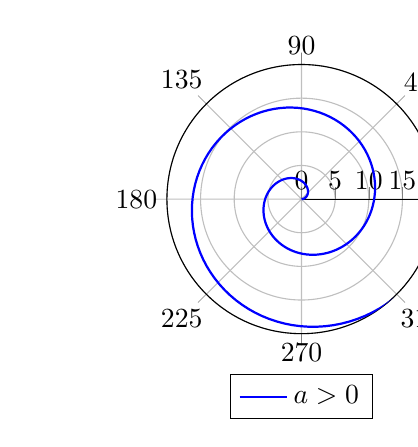
\begin{tikzpicture}
    \hspace{1cm}
    \begin{polaraxis}[
        width=5cm, 
        height=5cm,
        domain=0:720,
        ymax=20,
        samples=200,
        legend style={at={(0.5,-0.15)}, anchor=north},
    ]
    \addplot[blue, thick] {0.03*x}; 
    \addlegendentry{$a > 0$}
    \end{polaraxis}
    \hspace{7cm}
    \begin{polaraxis}[
        width=5cm, 
        height=5cm,
        domain=0:720, 
        ymax=20,
        samples=200,
        legend style={at={(0.5,-0.15)}, anchor=north},
    ]
    \addplot[blue, thick] {-0.03*x}; 
    \addlegendentry{$a < 0$}
    \end{polaraxis}
\end{tikzpicture}

\section{Polar Distance Formula}

Consider two points \(P(r_1, \theta_1)\) and \(Q(r_2, \theta_2)\) in polar coordinates.

Step 1: Convert to Cartesian coordinates:
\[
P: (x_1, y_1) = (r_1 \cos \theta_1, r_1 \sin \theta_1)
\]
\[
Q: (x_2, y_2) = (r_2 \cos \theta_2, r_2 \sin \theta_2)
\]

Step 2: Calculate the Cartesian distance \(d\) between \(P\) and \(Q\):
\[
d = \sqrt{(x_2 - x_1)^2 + (y_2 - y_1)^2}
\]

Step 3: Substitute the expressions for \(x_1\), \(y_1\), \(x_2\), and \(y_2\) obtained in Step 1:
\[
d = \sqrt{(r_2 \cos \theta_2 - r_1 \cos \theta_1)^2 + (r_2 \sin \theta_2 - r_1 \sin \theta_1)^2}
\]

Step 4: Expand and simplify the expression:
\begin{align*}
    d = \sqrt{r_2^2 \cos^2 \theta_2 - 2r_1r_2 \cos \theta_1 \cos \theta_2 + r_1^2 \cos^2 \theta_1 + r_2^2 \sin^2 \theta_2 - 2r_1r_2 \sin \theta_1 \sin \theta_2 + r_1^2 \sin^2 \theta_1}
\end{align*}

Step 5: Use the trigonometric identity \(\cos^2 \theta + \sin^2 \theta = 1\) to simplify further:
\[
d = \sqrt{r_2^2 + r_1^2 - 2r_1r_2(\cos \theta_1 \cos \theta_2 + \sin \theta_1 \sin \theta_2)}
\]

Step 6: Use the trigonometric identity \(\cos(\theta_2 - \theta_1) = \cos \theta_1 \cos \theta_2 + \sin \theta_1 \sin \theta_2\) to get the final polar distance formula:
\[
d = \sqrt{r_2^2 + r_1^2 - 2r_1r_2 \cos(\theta_2 - \theta_1)}
\]

Therefore, the polar distance formula is proven.

\section{Complex Numbers}

\subsection{Introduction}

A \textbf{complex number} refers to the combination of a real number and an imaginary number. Students may be familiar with complex numbers given in their \textbf{rectangular form} $z = a+bi$. 

In rectangular form, similarly to vectors, $a$ represents the real component of $z$, while $b$ represents the imaginary component of $z$. We can plot complex numbers just like we plot real numbers. The only alteration we must make is to the coordinate plane: instead of $x$ and $y$ axes, we use a real axis and imaginary axis respectively to form a \textbf{complex plane}. 

From this graphical standpoint, we can observe that a complex number has a length and angle associated with it, just like a real number's magnitude and direction. In the case of the complex number $z = a+bi$, we call the associated length $|z| = \sqrt{a^2+b^2}$ its \textbf{modulus}, and the associated angle Arg($z$) $= \arctan(\frac{b}{a})$ its \textbf{argument}. Generally, the domain of a complex number's argument is $[\pi, \-pi)$. The reasons for this specific restriction are rooted in complex analysis. 

With this observation in mind, students should realize that complex numbers can also be expressed in polar form. If we denote the modulus as $r$ and the argument as $\theta$, then have the following:

\[ z = a+bi &= r\cos\theta + ri\sin\theta = r(\cos\theta + i\sin\theta) \]

Due to the length of this expression, the quantity $\cos\theta + i\sin\theta$ is commonly referred to as cis($\theta$). Thus, we have:

\[ z = a+bi = r\text{cis}(\theta) \]

\subsection{Complex Operations}

Similarly to real numbers, we would like to be able to perform arithmetic operations on complex numbers. Depending on the operation, representing the complex number in rectangular or polar form may be preferable to the other. 

For the addition and subtraction of two complex numbers, rectangular form is advantageous, as the real components simply combine with each other, and the same happens with the imaginary components.

\[ z_1+z_2 = (a_1 + b_1i) + (a_2 + b_2i) = (a_1+a_2) + (b_1+b_2)i \]
\[ z_1-z_2 = (a_1 + b_1i) - (a_2 + b_2i) = (a_1-a_2) + (b_1-b_2)i \]

On the other hand, for multiplication and division of complex numbers, polar form is preferable to work with. This is due to the fact that multiplication causes the moduli of the numbers to multiply and the arguments of the numbers to add. 

\[ z_1z_2 = (r_1\text{cis}(\theta_1))(r_2\text{cis}(\theta_2)) = r_1r_2\text{cis}(\theta_1+\theta_2) \]
\[ \frac{z_1}{z_2} =  \frac{r_1\text{cis}(\theta_1)}{r_2\text{cis}(\theta_2)} = \frac{r_1}{r_2}\text{cis}(\theta_1-\theta_2)\]

\subsection{Complex Powers}

Note that taking a power of a number is simply equal to multiplying the same number by itself a certain number of times. Let us investigate squaring a complex number. Recall that multiplication causes the moduli of the numbers to multiply and the arguments of the numbers to add.

\[ z^2 = (r\text{cis}(\theta))(r\text{cis}(\theta)) = r^2\text{cis}(2\theta) \]

We can take it several steps further:

\[ z^3 = z^2z = (r^2\text{cis}(2\theta))(r\text{cis}(\theta)) = r^3\text{cis}(3\theta) \]
\[ z^4 = z^3z = (r^3\text{cis}(3\theta))(r\text{cis}(\theta)) = r^4\text{cis}(4\theta) \]
\[ z^5 = z^4z = (r^4\text{cis}(4\theta))(r\text{cis}(\theta)) = r^5\text{cis}(5\theta) \]
\[ \text{\dots} \]

This pattern holds for any integer power $n$, and is also known as \textbf{DeMoivre's Theorem}:

\[ \text{For integers } n \text{ and complex number }z = r\text{cis}(\theta)\text{, } z^n = r^n\text{cis}(n\theta).\]

Thus, integer powers of complex numbers can easily be calculated using polar form. This then raises the question of how fraction powers, or roots, are calculated.

\subsection{Complex Roots}
% roots of unity
Students may recall from algebra that polynomials of degree $n$ always have $n$ zeroes. However, as we know, not all of them are guaranteed to be real. For example, take the following equation:

\[ x^4 = 16 \]

It seems that there are only two solutions here, $x=2$ and $x=-2$. However, these are only the real solutions. There are actually two more solutions in the complex plane:

\[ x^2 = -4 \to x = \pm 2i\]

Thus, we can observe that there are always a total of $n$ $n$-th roots of a complex number. For example, there are always two square roots, three cube roots, four fourth roots, etc. They are given by the following twist on DeMoivre's Theorem:\\

\begin{center}
For integers $n$ and complex number $z = r\text{cis}(\theta)$, $z^{\frac{1}{n}} = r^{\frac{1}{n}}\text{cis}(\frac{\theta+2\pi a}{n}\theta)$, where $a = 0, 1, 2, 3 \text{\dots} n-1$.
\end{center} 
\vspace{0.5 cm}

The $n$ $n$-th roots of 1 are referred to as the $n$-th \textbf{roots of unity}. Roots of unity and other complex roots can be found with the formula above. Additionally, the improper fraction powers of complex numbers can be found using a combination of DeMoivre's Theorem and the formula above.

\end{document}